% do not change these two lines (this is a hard requirement
% there is one exception: you might replace oneside by twoside in case you deliver 
% the printed version in the accordant format
\documentclass[a4paper, 11pt,titlepage,oneside,openany]{book}
\usepackage{times}


\usepackage{graphicx}
\usepackage{latexsym}
\usepackage{amsmath}
\usepackage{amssymb}
\usepackage{subfigure}
\usepackage{verbatim}
\usepackage{listings} 
\usepackage{booktabs}
\lstset{language=Python,
	basicstyle=\ttfamily\scriptsize,
	breaklines=true}    
\usepackage{glossaries}          
\usepackage{ntheorem}
\usepackage{caption}
\DeclareCaptionType{code}[Algorithm][List of Code] 
% \usepackage{paralist}
\usepackage{tabularx}
\usepackage{amsmath}
% this packaes are useful for nice algorithms
%\usepackage{algorithm}%;, algorithmic}
\usepackage[linesnumbered,ruled,vlined]{algorithm2e}
\SetKwInput{KwIn}{Input}                % Set the Input
\SetKwInput{KwOut}{Output}              % set the Output
\AtBeginEnvironment{algorithm}{\scriptsize}
\AtBeginEnvironment{tabular}{\scriptsize}
\AtBeginEnvironment{amsmath}{\scriptsize}
%\usepackage{algorithmic}
\usepackage{array}
\usepackage{multirow}
\usepackage{url}


\newcommand\MyBox[2]{
	\fbox{\lower0.75cm
		\vbox to 1.7cm{\vfil
			\hbox to 1.7cm{\hfil\parbox{1.4cm}{#1\\#2}\hfil}
			\vfil}%
	}%
}

% well, when your work is concerned with definitions, proposition and so on, we suggest this
% feel free to add Corrolary, Theorem or whatever you need
\newtheorem{definition}{Definition}
\newtheorem{proposition}{Proposition}


% its always useful to have some shortcuts (some are specific for algorithms
% if you do not like your formating you can change it here (instead of scanning through the whole text)
%\renewcommand{\algorithmiccomment}[1]{\ensuremath{\rhd} \textit{#1}}
\def\MYCALL#1#2{{\small\textsc{#1}}(\textup{#2})}
\def\MYSET#1{\scshape{#1}}
\def\MYAND{\textbf{ and }}
\def\MYOR{\textbf{ or }}
\def\MYNOT{\textbf{ not }}
\def\MYTHROW{\textbf{ throw }}
\def\MYBREAK{\textbf{break }}
\def\MYEXCEPT#1{\scshape{#1}}
\def\MYTO{\textbf{ to }}
\def\MYNIL{\textsc{Nil}}
\def\MYUNKNOWN{ unknown }
% simple stuff (not all of this is used in this examples thesis
\def\INT{{\mathcal I}} % interpretation
\def\ONT{{\mathcal O}} % ontology
\def\SEM{{\mathcal S}} % alignment semantic
\def\ALI{{\mathcal A}} % alignment
\def\USE{{\mathcal U}} % set of unsatisfiable entities
\def\CON{{\mathcal C}} % conflict set
\def\DIA{\Delta} % diagnosis
% mups and mips
\def\MUP{{\mathcal M}} % ontology
\def\MIP{{\mathcal M}} % ontology
% distributed and local entities
\newcommand{\cc}[2]{\mathit{#1}\hspace{-1pt} \# \hspace{-1pt} \mathit{#2}}
\newcommand{\cx}[1]{\mathit{#1}}
% complex stuff
\def\MER#1#2#3#4{#1 \cup_{#3}^{#2} #4} % merged ontology
\def\MUPALL#1#2#3#4#5{\textit{MUPS}_{#1}\left(#2, #3, #4, #5\right)} % the set of all mups for some concept
\def\MIPALL#1#2{\textit{MIPS}_{#1}\left(#2\right)} % the set of all mips



\makeglossaries

\begin{document}

\pagenumbering{roman}
% lets go for the title page, something like this should be okay
\begin{titlepage}
	\vspace*{2cm}
  \begin{center}
   {\Large Hyperpartisan News Detection\\}
   \vspace{2cm} 
   {Bachelor Thesis\\}
   \vspace{2cm}
   {presented by\\
    Larissa Strauch \\
    Matriculation Number 1518629\\
   }
   \vspace{1cm} 
   {submitted to the\\
    Data and Web Science Group\\
    Prof.\ Dr.\ Ponzetto\\
    University of Mannheim\\} \vspace{2cm}
   {Juli 2019}
  \end{center}
\end{titlepage} 

% no lets make some add some table of contents
\tableofcontents
\newpage

\listofalgorithms
\listoffigures

\listoftables

\newglossaryentry{tf}
{
	name=TF,
	description={Term Frequency}
}
\newglossaryentry{idf}
{
	name=IDF,
	description={Inverse Term Frequency}
}
\newglossaryentry{tfidf}
{
	name=TF-IDF,
	description={Term Frequency-Inverse Term Frequency}
}
\newglossaryentry{bert}
{
	name=BERT,
	description={Bidirectional Encoder Representations from Transformers}
}
\newglossaryentry{cbow}
{
	name=CBOW,
	description={Continous Bag of Words}
}
\newglossaryentry{mnb}
{
	name=Multinomial NB,
	description={Multinomial Naives Bayes}
}


\printglossaries %in cmd for printing: makeindex -s BA.ist -t BA.glg -o BA.gls BA.glo

% evntuelly you might add something like this
% \listtheorems{definition}
% \listtheorems{proposition}

\newpage


% okay, start new numbering ... here is where it really starts
\pagenumbering{arabic}

\chapter{Introduction}

\section{Problem Statement}
 
 

\section{Contribution}

 

\section{Related Work}

\chapter{Fundamentals}

\section{Term Frequency-Inverse Document Frequency}
Term frequency (\gls{tf}) is a measure that denotes how frequently a term \textit{t} appears a the document \textit{d}. One way to compute \gls{tf} is \cite{IR-book}:\\
\[
tf(t,d)=\frac{1+\log(tf_{t,d})}{1+\log(ave_{t\in d}(tf_{t,d}))}
\]
where $1+\log(tf_{t,d})$ reflects how many times the term $t$ appears in document $d$ and $1+\log(ave_{t\in d}(tf_{t,d}))$ is the highest occurrence of any term in document $d_i$.\\

\noindent Inverse Doucment Frequency (\gls{idf}) points to the assumption that the informativeness of the term \textit{t} is inversely proportional to the number of documents in the collection in which the term appears \cite{IR-book}.\\
\[
idf(t_i)=log\frac{N}{d \in D : t \in d}
\]
Where $N$ is the total amount of doucments in a document set and $d \in D : t \in d$ is the amount how many times the term $t$ appears in the document set.\\

\noindent To compute the weight for the term $t_i$ within the document $d_j$ we simply multiply the \textit{TF} and \textit{IDF} components:
\[
w_{ij}=tf(t_i, d_j)\cdot idf(t_i)
\]
Therefore, \Gls{tfidf} indicates how significant a word is to a document in a collection or corpus. It is regularly used as a weighting factor in Information Retrieval and Text Mining. The \Gls{tfidf} value increases proportionally to the number of times a word appears in the document, but is offset by the frequency of the word in the corpus, which helps to control the fact that some words are usually more common than others.\\
\noindent \Gls{tfidf} is easy to compute. In addition, it is possible to extract the most descriptive terms, as well as to calculate the similarity between 2 terms. However, TF-IDF is based on the bag-of-words (BoW) model, which is why it disregards aspects such as text position, semantics and co-occurrence.

\section{Word Embeddings}
Word Embeddings are based on the approach of Harris Distributional Hypothesis \cite{distributionalhypothesis} from 1951, which states, that words that occur in the same contexts tend to have similar meanings. \\
\noindent A Word Embedding provides a word vector for each word. This is done by extracting features from that word within the context in which it appears and assigning it a place within the vector space. Two similar words will occupy locations areas near one another within this vector space, while words that differ will have positions much further apart. This makes it possible to calculate the distance calculation by computing cosine distance.

\subsection{Word2Vec}
Word2Vec is a "2-Model Architecture for computing continuous vector representations of words from very large dataset"\cite{effiecientestimation} that creates an n-dimensional vector space in which each word is represented as a vector. Word2Vecs 2 learning models are the \gls{cbow} and Skip-Gram-Model.\\
\\
\noindent \gls{cbow} uses the context word to predict the target word. The input is a one-hot encoded vector. The weights between the input layer and the output layer can be represented by a $V \cdot N$ matrix \textit{W} where "each row of $W$ is the $N$-dimension vector representation $w_v$ of the associated word of the input layer" \cite{word2vecparam}. The hidden-layer \textit{h} is computed by multiplying the one-hot encoding vector of the input word $w_I$ with the weight matrix \textit{W} \cite{word2vecparam}.
\[
h=W^Tx=W_{(k, \cdot)}^{T}:=v_{w_I}^{T}
\] 
Next we have another weight matrix $W'={w'_{ij}}$ which is an $N \cdot V$ matrix. With these weights we can finally compute a score $u_j$ for each word in the vocabulary \cite{word2vecparam}
\[
u_{j}={v'}_{w_j}^{T}h
\] where ${v'}_{w_j}$ is the \textit{j}-th column of the matrix \textit{W'}. Afterwards "we can use \textit{softmax}, which is a log-linear classification model, to obtain the posterior distribution of words" \cite{word2vecparam}.
\[
p(w_j|w_I)=y_j=\frac{exp(u_j)}{\sum_{j'=1}^V exp(u_{j'})}
\] \\
\\
\noindent In contrast to the \gls{cbow} model,  Skip-Gram uses the target word to predict the context words. The input is still a one-hot encoding vector, the hidden layers definition stays the same as in the \gls{cbow} model, each output is still using the same hidden layer to output matrix as in the \gls{cbow} model $p(w_{c,j}=w_{O,c}|w_I)=y_{c,j} = p(w_j|w_I)=y_j$ and the function for $u_j=u_{c,j}$ stays the same \cite{word2vecparam}. However in the output layer, we are now outputting \textit{C} multinomial distributions. 
\section{SVM}
\section{Multinomial Naive Bayes Classifier}
The Naive Bayes classifier is based on  Bayes' theorem, which comes from the probability calculus and describes the calculation of conditional probability. Each object in this classification approach is assigned to the class for which the highest probability was computed or for which the lowest costs arise in this assignment.  \\
\noindent The Multinomial Naive Bayes classifiers assumes that the position of the word does not matter, as well as  that the feature probabilities $P(x_i|c_j)$ are independent given a class $c$.
"The probability of a class value $c$ given a test document $d$ is computed as
\[
P(c|d)=\frac{P(c)\prod \limits_{w \in d}P(w|c)^{n_{wd}} }{P(d)}
\]
where $n_{wd}$ is the number of times word $w$ occurs in document $d$, $P(w|c)$ is the probability of observing word $w$ given class $c$, $P(c)$ is the prior probability of class $c$, and $P(d)$ is a constant that makes the probabilities for the different classes sum to one". [https://link.springer.com/content/pdf/10.1007\%2F11871637.pdf]
\section{Logistic Regression Classifier}
\begin{figure}[h]
	\centering
	%Arbeit:
	%includegraphics[width=0.5\textwidth]{C:/Users/lastrauc/Documents/Git/ThesisPaper/Pictures/Hypeprartisan_LabeledByPublisher.png}
	%PC:
	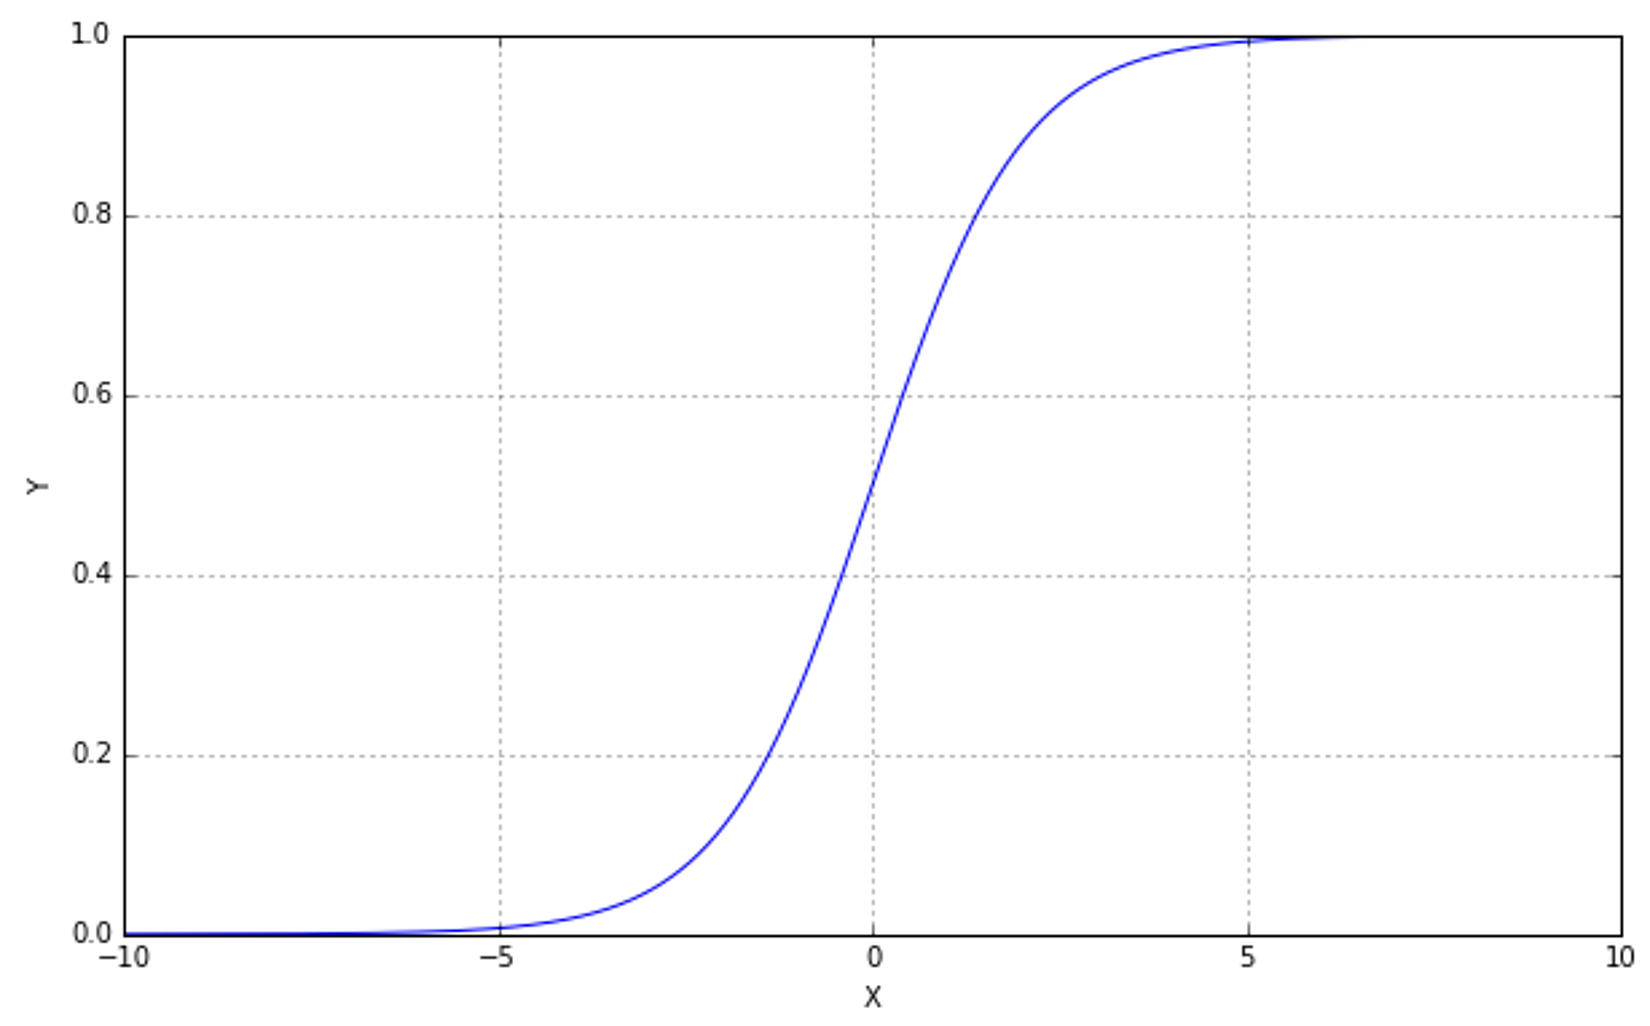
\includegraphics[width=0.5\textwidth]{C:/Users/Laris/Documents/Bachelorarbeit/Git/ThesisPaper/Pictures/sigmoid.png}
	%Lap Top:
	%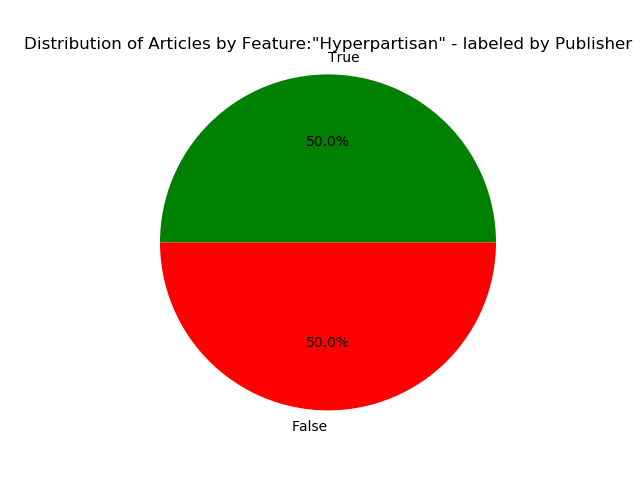
\includegraphics[width=0.5\textwidth]{C:/Users/Larissa/Documents/Uni/Bachelorarbeit/Git/ThesisPaper/Pictures/Hypeprartisan_LabeledByPublisher.png}
	\caption{sigmoid function[Machine learning algorithms : reference guide for popular algorithms for data science and machine learning
		]}
	\label{fig:example}
\end{figure}
\noindent Logistic Regression is like Naive Bayes, a probabilistic classifier, and thus classifies by estimating the probability $P(Y|X)$ that the object belongs to a particular class.
It can be derived analogously to the linear regression hypothesis, 
\[
h_\Theta(x)=\Theta_0+\Theta_1x_1+...+\Theta_nx_n=\sum_{i=0}^{n}\Theta_ix_i=\Theta^\tau x
\]
where $h_\Theta(x)$ is the predicted value, $\Theta$ is the model's parameter vector, $\Theta_0$ is the bias term and $x_i$ is a feature of feature vector. The logistic regression hypothesis generalizes the linear one to use the logistic function
\[
h_\Theta(x)=s(\sum_{i=0}^{n}\Theta_ix_i)=s(\Theta^\tau x)
\]
and in contrast to linear regression, in logistic regression only values between 0 and 1 are obtained, which can be attributed to the addition of the sigmoid function (Figure 2.1). 
\[
s(x)=\frac{1}{1+e^{-x}}
\]
Combining these two therefore results in
\[
h_\Theta(x)=\frac{1}{1+e^{-\Theta^\tau x}}
\]
\noindent To find the optimal $\Theta$ by which we get an $h_\Theta(x)$ that is close to 0 or 1, we maximize the log-likelihood relying upon the output class, therefore the optimization problem can be expressed, utilizing the indicator notion as the minimization of the loss function\cite{algorithms}:
\[
l(\Theta)=-\sum_{i=1}^{n}y_i\ln(z_i)+(1-y_i)\ln(1-z_i) \qquad ,\forall i,y_i \in {\{0,1\}} \\
\]
where $z=h_\Theta(x)$. \\
\noindent This implies, if $y=0$, the first term ends up $0$ and the second $\ln(1-z)$, which results in a log-likelihood of $0$. In the event that $y=1$, the second term ends up 0 and the first one corresponds to the log-likelihood of $z$. Along these lines, both cases are integrated into a solitary articulation. \\
\noindent A major issue in machine learning is the aspect of overfitting. Overfitting tends to adjust the model too much to the training data. This happens when a model learns the details in the training data so that the performance of the model is contrairily influenced by new data. This implies that noise or random fluctuations in the training data are recorded and learned as concepts by the model. The issue is, that these concepts do not apply to new data and negatively impact the generalization of the model. Therefore, there is the process of \textit{regularization}, which is a form of regression that decreases the coefficient estimation to $0$ and assumes that smaller weights generate simpler models and thus helps avoid overfitting. \\
\noindent Two of the most commonly used regression techniques are \textit{Lasso Regression (L1)} and \textit{Ridge Regression (L2)}, which differ mainly in the penalty term. \\
\noindent The \textit{L1} loss function minimizes the sum of the absolute differences between the target value and the estimated values. If input characteristics have weights closer to zero, this results in a sparse L1 standard. In the Sparse solution, most of the input features have zero weights and very few features have non-zero weights. The L1 regulation offers a function selection. This is done by associating insignificant input features with zero weights and useful features with a non-zero weight.  In the L1 control, we punish the absolute value of the weights. It is defined as:
\[
||w||_1=\sum_{i}^{n}|w_i|
\]
Which we add to the loss function:
\[
l_\lambda^R(\Theta)=-\sum_{i=1}^{n}y_i\ln(z_i)+(1-y_i)\ln(1-z_i)+\lambda\sum_{j=1}^{p}|w_j|
\]
The L2 loss function is essentially about minimizing the sum of the square of the differences between the nominal value and the estimated values.
L2 control forces the weights to small weights, but does not make them zero and leads to a not sparse solution. In addition, L2 is not robust against outliers, since square terms inflate the error differences of the outliers and the regularization term tries to correct them by punishing the weights. It is defines as follows:
\[
||w||_2^2=\sum_{i}^{n}w_i^2
\]
,which we add as well to the loss function:
\[
l_\lambda^L(\Theta)=-\sum_{i=1}^{n}y_i\ln(z_i)+(1-y_i)\ln(1-z_i)+\lambda\sum_{j=1}^{p}|w_i^2|
\]

\section{Decision Trees and Random Forest Classifier}
\subsection{Decision Trees}
Starting from the root node of a tree, a feature is evaluated from which a branch is subsequently selected. This process is repeated until the last node in the tree (leaf) is reached, which supplies the corresponding class. Different approaches have been developed in Decision Trees. One of the first is called \textit{Iterative Dichotomizer (ID3)} and required explicit features. This condition led to the development of the \textit{C4.5} formulation, which also manages continuous (but summarized and discretized) values. In addition, C4.5 was also known for its ability to transform a tree into a series of conditional expressions. The latest development is called \textit{Classification and Regression Trees (CART)}. These kinds of trees can oversee both downright and numeric highlights, can be utilized in either characterization or relapse assignments, and don't utilize a standard set as an inner portrayal\cite{algorithms}.\\
\noindent The algorithm uses impurity measures to select a particular branch from a leaf. Among others, the two most common measures are "Gini" and "Cross Entropy Index"\cite{algorithms}.  These impurity measures are  applied to each candidate subset, and the resulting values are combined (e.g., averaged) to provide a measure of the quality of the split,
\[
I_{Gini}(j)=\sum_{i}p(i|j)(1-p(i|j))
\]
\[
I_{Cross-entropy}(j)=-\sum_{i}p(i|j)log(p(i|j))
\]
where $j$ is a certain node, $p(i|j)$ is the probability with $i \in [1,n]$ associated with each class.\\
\noindent The \textit{Gini} Index measures the impurity based on the likelihood of misclassification if a sample is categorized using a label randomly chosen from the node subset distribution. The minimum index (0,0) is achieved when all examples are characterized into a solitary class.\\
\noindent \textit{Cross-Entropy} depends on information theory, and accepts invalid qualities just when samples having a place with a solitary class are available in a split, while it is greatest when there's a uniform conveyance among classes.

\subsection{Random Forest Classifier}
The Random Forest classifier is a classification technique that creates multiple decision trees from randomly selected subsets of training data. Each tree in this process may make a decision, these votes are then aggregated to determine the final class. According to Breiman \cite{randomforest} the Random Forest algorithm is as follows:\\

\begin{algorithm}[H]
	\DontPrintSemicolon
	Set the number of decision trees $N_c$\;
	\For{$i\gets 1$ \KwTo $N_c$}
		{Create a dataset $D_i$ sampling with replacements from the original dataset $X$}
	Set the number of features  to consider during each split $N_f$\;
	Set an impurity measure\;
	Define an optimal maximum for each tree\;
	\For{$i\gets 1$ \KwTo $N_c$}
		{Random Forest: Train the decision tree $d_i(x)$ using the dataset $D_i$ and selecting the best split among \textit{Nf} features randomly sampled \\
		Extra-trees:  Train the decision tree $d_i(x)$ using the dataset $D_i$ computing before each split $n$ random thresholds and selecting the one that yield the least impurity}
	Define an output function averaging the single outputs or employing a majority vote
	\caption{Random Forest}
\end{algorithm}
\section{Cross Validation}
\textit{Cross Validation} is a model validation technique used to survey how the result of measurable statistical analysis generalizes into an independent dataset. The idea is to divide the entire dataset into a moving test and training set. The size of the test set is determined by the quantity of folds, so that at \textit{k} emphases the test set covers the whole original dataset.\\
\noindent A round of \text{Cross Validation} comprises of separating a sample of data into corresponding subsets, performing the analysis on the training set, and validating the analysis on the test set. To decrease fluctuation, most strategies perform several rounds of \textit{Cross Validation} utilizing various partitions and combine the validation result over the rounds to obtain an estimate of the predictive performance of the model.
\section{Evaluation}
In order to evaluate how well a classifier works, several procedures exist. The ones used during the competition are \textit{Accuracy}, \textit{Recall}, \textit{Precision} and \textit{F1-Score}, for which the Confusion Matrix (Table 2.1) forms the basis. Each column of the matrix represents the instances of a predicted class, while each row represents the instances of the actual class. \\
\begin{center}
	\renewcommand\arraystretch{1.5}
	\setlength\tabcolsep{0pt}
	\begin{tabular}{c >{\bfseries}r @{\hspace{0.7em}}c @{\hspace{0.4em}}c @{\hspace{0.7em}}l}
		\multirow{10}{*}{\parbox{1.1cm}{\bfseries\raggedleft Actual\\ Class}} & 
		& \multicolumn{2}{c}{\bfseries Predicted Class} & \\
		& & \bfseries positive & \bfseries negative \\
		& positive$'$ & \MyBox{True}{Positives} & \MyBox{False}{Negatives} \\[2.4em]
		& negative$'$ & \MyBox{False}{Positives} & \MyBox{True}{Negatives} \\
	\end{tabular}
	\captionof{table}{Confusion Matrix}
\end{center}
\noindent \textit{True Positive} means that the classifier predicted a class which actually corresponds to it, whereas \textit{False Positive} means that a class was predicted that does not correspond to the actual class. In contrast, there are the \textit{False Negatives}, where the classifier predicted a class as not belonging, although the instance actually belongs to it whereas \textit{True Negative} means that the class was correctly classified as not belonging. \\
\noindent The four evaluation metrics are computed as follows \cite{algorithms}:
\begin{itemize}
	\item Accuracy: $\frac{TP+TN}{TP+TN+FP+FN}$\\
					Defines the correct classification to the total number of cases
	\item Precision: $\frac{TP}{TP+FP}$\\
	Defines the correct classification of cases predcited to be positive
	\item Recall: $\frac{TP}{TP+FN}$\\
	Defines the correct positive classification of cases that are actually positive
	\item F1-Score: 2 $\cdot$ $\frac{Precision \cdot Recall}{Precision+Recall}$\\
	Defines the average of precision and recall,
	where an F1 value reaches its best value at 1
	and worst at 0
\end{itemize}
\chapter{Data}
\label{cha:theory}


\section{Data Description}
 The given data, on which we want to build our model on, was provided by zenodo.org as part of SemEvals Task 4 [Link zu Task hinzufügen]and consists of 2 independent datasets, which in turn have been divided into a GroundTruth-, Training- and Validation set.
 
 \noindent The first dataset, recognizable by the term 'byPublisher', reflects the publisher's general bias set forth by BuzzFeed journalists or MediaBiasFastCheck.com beforehand. It consists of a total of 750,000 items, of which 600,000 belong to the Training- and 150,000 to the Validation set.
 
 \noindent In return, the second dataset, recognizable by the term 'byArticle', was scrapped by crowdsourcing at hand and therefore consists of only 645 items without a Validation set.\\
 \\
The GroundTruth-, Validation- and Training sets were each provided as XML documents. The GroundTruth file contains the attributes \textit{article-url}, \textit{labeled-by}, \textit{id} and \textit{hyperpartisan}. The main distinction between the by Article and by Publisher labelled datasets is that the by Publisher labelled GroundTruth dataset contains an additional attribute named \textit{bias}. In this context, the \textit{article-url} provides the URL of the article, the characteristic \textit{labeled-by} reflects whether the article belongs to the publisher or article dataset, \textit{id} represents a unique ID for the article, Hyperpartisan reflects whether the article was labeled als Hyperpartisan or not and the additional attribute \textit{bias} in the publisher record, states whether the article belongs to the "left", "left-center", "least", "right-center" or "right" sector.
 

\subsection{Dataset labelled by Publisher}
\begin{minipage}[T]{.45\linewidth}
	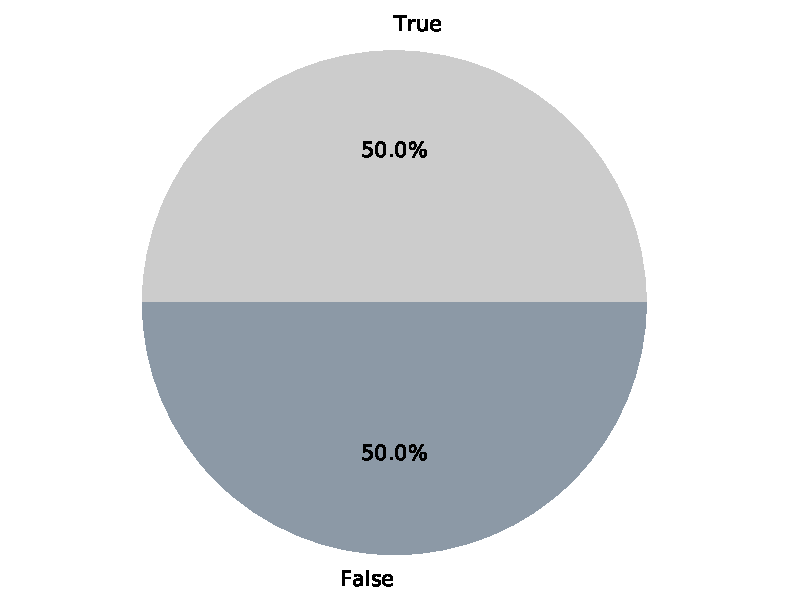
\includegraphics[width=\linewidth]{C:/Users/Laris/Documents/Bachelorarbeit/Git/ThesisPaper/Pictures/hyper_pub.pdf}
	\captionof{figure}{Hyperpartisan Distribution by Publisher}
\end{minipage}
	\hspace{.1\linewidth}% Abstand zwischen Bilder
\begin{minipage}[T]{.45\linewidth}
	\centering
	\begin{tabular}{ccc}
		\toprule
		Publisher & Bias & Amount \\
		\midrule
		Fox Business & Left & 96175 \\
		CounterPunch & Left & 39832 \\
		Mother Jones & Left & 36730 \\
		Truthdig & Left & 25056 \\
		Daily Wire & Right & 18570 \\
		\bottomrule
	\end{tabular}
	\captionof{table}{Publishers with the highest proportion of Hypeprartisan articles}
\end{minipage}\\
\\ As mentioned above, this dataset consists of a total of 750,000 articles and is divided into a training record consisting of 600,000 articles and a validation set consisting of 150,000 articles.
The main difference between this dataset and the by articel labelled one is the type of classification. This is because these articles were not labelled as Hyperpartisan based on their content, but due to the publisher (Table 3.1). This means, that a publisher who has been designated as right or left by the MediaBiasFastCheck.com will naturally publish articles which are Hyperpartisan. This manifests itself in a different form of features, which becomes apparent in the further course of this thesis. This likewise influences the distribution of Hyperpatisan articles.
 Out of a total of 750,000 items, 375,000 assume the value 'True', while the remaining 375,000 have the value 'False'(Figure 3.1). 
Furthermore, the classification is expressed by the distribution of the additionally contained GroundTruth attribute 'Bias', which informs about the general bias of the publisher. All 375,000 Hyperpartisan labelled all are assigned to either the left or right sectors, but none are right-centre, least or left-centre and are again 50:50 distributed. The other 50\% are split between the remaining bias, with 'Least' owning the largest share at 37\%.\\
The publicity data is distributed over the years 1964-2018, with most of the data coming from 2012-2018.


\subsection{Dataset labelled by Article}

As already described in the previous section, the distribution of the by Article dataset is different from the by Publisher one. The distribution is no longer 50:50, but only 36.9\% were classified as Hyperpartisan. 
\begin{figure}[t]
	\begin{minipage}{.45\linewidth}
		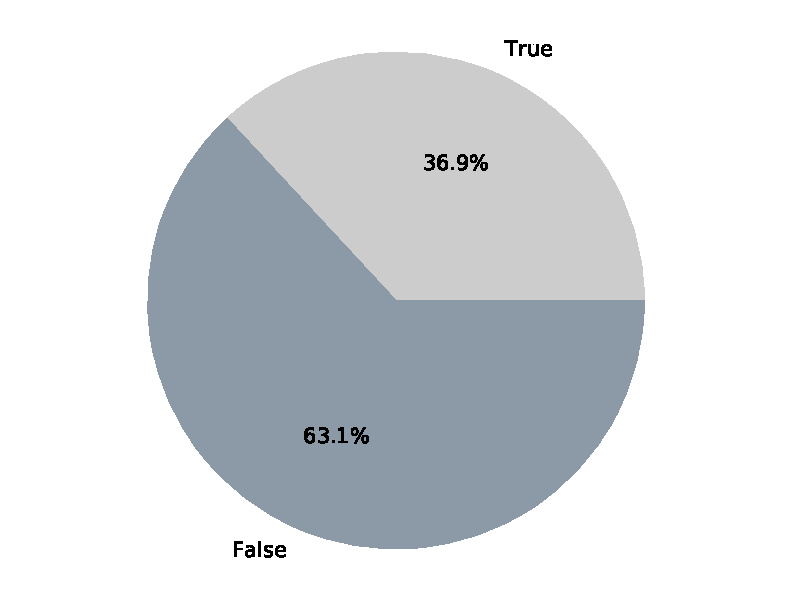
\includegraphics[width=\linewidth]{C:/Users/Laris/Documents/Bachelorarbeit/Git/ThesisPaper/Pictures/figure2.pdf}
		\caption{Hyperpartisan Distribution by Article}
	\end{minipage}
	\hspace{.1\linewidth}% Abstand zwischen Bilder
	\begin{minipage}{.45\linewidth}
	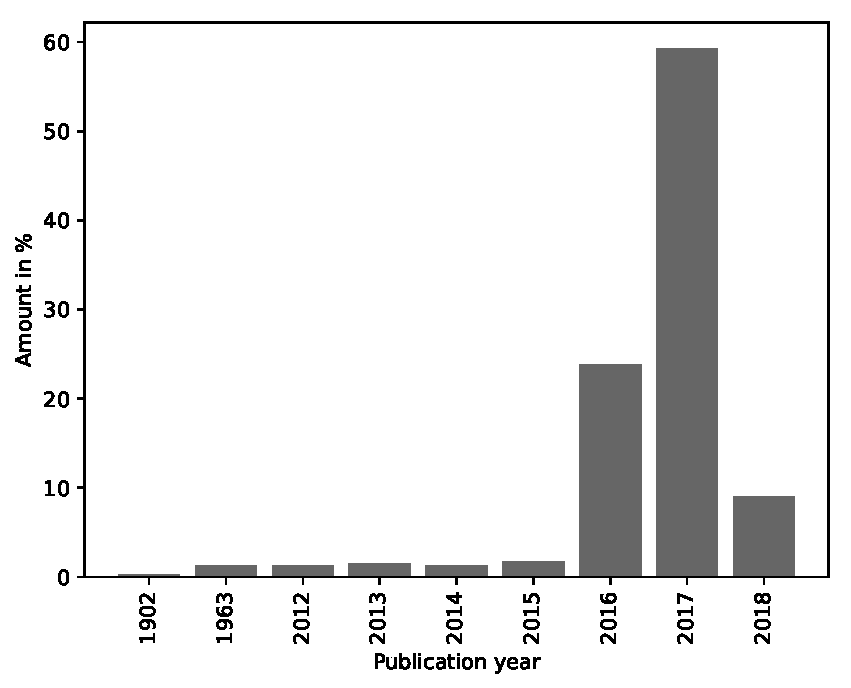
\includegraphics[width=\linewidth]{C:/Users/Laris/Documents/Bachelorarbeit/Git/ThesisPaper/Pictures/figure.pdf}
	\caption{Publishing Years Distribution by Article}
\end{minipage}
\end{figure}
\noindent Here we can see that there is no more 50:50 distribution. Only 36.9\% were defined here as Hyperpartisan as shown in figure 3.2.\\
\noindent Moreover, in this dataset, the distribution of publication data is not mainly from the years 2012-2018, but in 2016-2018, with the largest number of articles dating back to 2017 at just under 60\% as we can see in figure 3.3. Altogether all 645 articles date from the years 1902-2018.




\section{Data Preparation}
In order to be able to work with the existing data in the further course of this project, several preprocessing steps are necessary. In the preprocessing phase of my bachelor's thesis, the data therefore went through the following steps:
\begin{enumerate}
	\item File Parsing. 
	\item Information Filtering.
	\item Combine Data.
	\item Special Characters and Stop Word Removal.
	\item Tokenization and Stemming.
\end{enumerate}	
\noindent As a result, in the following section, I will go further into detail how I preprocessed my data.


\subsection{File Parsing}
Since it is difficult to work with the given data in an XML format, the first challenge is to convert these files into a format which allows it to work with them more easily. The particular challenge here is the size of the dataset labelled by publisher. A standard algorithm for reading XML files is provided by pythons DOM library \textit{ElementTree}, called \textit{ElementTree.parse}\cite{parse}. This method returns an ElemenTree type, which "is a flexible container object, designed to store hierarchical data structures in memory" [ http://effbot.org/zone/element.htm]. Meaning, that this library forms the entire model in the memory which can pose a problem with very large files, such as ours. As a substitute, I therefore use the method \textit{ElemenTree.iterparse}, which can process XML documents in a streaming fashion, retaining in memory only the most recently examined parts of the tree\cite{iterparse}. 


\subsection{Information Filtering}
As mentioned in Chapter 2.1 Data Description, the XML files include various features, which is why it is necessary to extract these features from XML file. In order to be able to do this, we pass an algorithm the, by the \textit{iterparse} method read content, which then passes through this algorithm in a double for-loop and checks for each item of an element in the content which "key" is currently processed. I then save this in an array, so that the features which have already been parsed, can be used later. \\

\begin{algorithm}[H]
	\DontPrintSemicolon
	\caption{Parse Ground-Truth File}
	\KwIn{Ground-Truth File}
	\KwOut{Trained Classifier} 
	\For{event, elem in content}
		{
		\For{key, value in elem.items()}
			{
			\uIf{key == 'id'}
				{id\_array.append(str(value))}
			\uElseIf{key == 'published-at'}
				{published\_at\_array.append(value)}
			\uElseIf{key == 'title'}
				{title\_array.append(value)}
			}
		}
\end{algorithm}

\subsection{Combine Data}
Since both, the Groundtruth- and Trainingdata contain important information, it is necessary to merge them into one file. I decided to use Python's library \textit{pandas} \cite{pandas} to combine both files into a single one. This, and especially Pandas, allows us to read the file more quickly as well as to access individual rows and columns of the merged file in a targeted manner.\\

\begin{algorithm}[H]
	\DontPrintSemicolon
	\caption{Merge Groundtruth- and Trainingdatasets}
	content = content\_parser.parse\_content(content\_training)\;
	a\_id = feature\_extraction.get\_id\_array()\;
	\BlankLine
	\BlankLine
	published = feature\_extraction.get\_published\_at\_array()\;
	title = feature\_extraction.get\_title\_array()\;
	bias = groundtruth\_parser.get\_bias\_array()\;
	hyperpartisan = groundtruth\_parser.get\_hyperpartisan\_array()\;
	\BlankLine
	columns = \{"ArticleID": a\_id, "PublishedAt": published, "Title": title, "Bias": bias, "Content": content  "Hyperpartisan": hyperpartisan\}\;
	\BlankLine
	\BlankLine
	tf = Pd.DataFrame(columns)\;
	tf = tf[['ArticleID','Published', Title','Bias','Content','Hyperpartisan']]\;
	tf.to\_csv(titlecsv,encoding='utf-8',index=False)\;
\end{algorithm}

\subsection{Special Characters and Stop Word Removal}
Since the GroundTruth- and Trainingdatasets have been combined into a single file, the next step  is to remove special characters and stop words. Especially the removal of stopwords is necessary since not all words presented in a document, such as auxiliary verbs, conjunctions and articles \cite{textclassification} are useful for training a classifier.\\

\begin{algorithm}[H]
		\DontPrintSemicolon
	stop = stopwords.words('english')\;
	\BlankLine
	\BlankLine
	df['Content'] = df['Content'].apply(lambda x: ''.join([item for item in x.split() if item not in stop]))\;
	df['Content'] = df['Content'].map(lambda x: re.sub(r"[\^ a-zA-Z0-9]+", '', x))\;
	\caption{Remove special characters and stop words}
\end{algorithm}
\noindent Here it becomes obvious that using pandas was a good choice, as we can now specifically access the 'Content' and 'Title' columns in order to perform this step of preprocessing on only these two and not the whole file.


\subsection{Tokenization and Stemming of the datasets}
After cleaning the dataset, the words are tokenized in order to convert them into numerical vectors so that a classifier is able to work with them. Tokenization is definied as "The process of demarcating and possibly classifying sections of a string of input characters. The resulting tokens are then passed on to some other form of processing. The process can be considered a sub-task of parsing input.\\
\noindent Stemming is the procedure of reducing the word to its grammatical root. The result is not necessarily a valid word of the language. For example, "recognized" would be converted to "recogniz". Still, the basic word almost always contains the very meaning of the word. Stemming is advantageous in that the algorithm used later now only has to fall back on a few different words and instead of many, all of which have the same meaning.\\
\\
\noindent In order to implement Stemming and Tokenization, only 2 lines of python code are necessary, due to the Pandas dataframe. \\

\begin{algorithm}[H]
	\DontPrintSemicolon
	df.Content = df.Content.apply(nltk.word\_tokenize)\;
	df.Content = df.Content.apply(lambda x: [stemmer.stem(y) for y in x])\;
	\caption{Special Character and Stopword Removal with Pandas and NLTK}
\end{algorithm}

\chapter{Methodology}
The primary procedure in Text Classification consist of 6 steps. These include  reading the dataset, tokenization, stemming, removing stop words, represent the text using vectors, as well as applying classification algorithms. Since the first four steps have already been covered in Chapter 2, I will discuss the remaining 3 in this section. Especially, step 6 plays an important role. As already mentioned in Chapter 1 - Introduction, we build the classifier using \glspl{bert}-Embeddings. In order to compare how the model performs, I will therefore focus on classical text classification algorithms.

%\section{Important Algorithms}
%In order to avoid the repetition of algorithms used in the same context, in this section, I will explain some recurring algorithms.
%\begin{algorithm}
%	\DontPrintSemicolon
%	import pickle\;
%	filename = 'finalized\_model.sav'\;
%	pickle.dump(model, open(filename, 'wb))
%	\caption{Saving a trained model}
%\end{algorithm}
%\begin{algorithm}
%	\DontPrintSemicolon
%	loaded\_model = pickle.load(open(filename, 'rb'))
%	\caption{Loading a trained model}
%\end{algorithm}

\section{Vector Representation of the Text}
In order for our classifier to be able to work with the text, we first need to transform our words into a feature vector representation. A document is a sequence of words [Text Categorization with Support Vector Machines] so a document can be presented by a One-Hot encoded vector, assigning the value 1 if the document contains the feature-word or 0 if the word does not appear in the document\cite{textclassification}. However, using this technique for word representation, resolves in a $V \cdot V$ Matrix, as we have V-diemensional vertor for each out of V words which can lead to huge memory issues. In addition this does not notion similiarity between words. Therefore I will go into further detail for better approaches in the next 2 subchapters.

\subsection{Term Frequency-Inverse Document Frequency}
A comparative approach I used in the course of my Bachelor Thesis is Term Frequency-Inverse Document Frequency. By using \gls{tfidf}, we're able to represent a word as a vector by assigning it weight which is computed through Term-Frequency multiplied with Inverse-Term-Frequency. Table 4.1 shows the 10 terms which have been assigned the highest \gls{tfidf} weights. Python's library \textit{scikit-learn}\cite{scikit-learn} provides two ways to implement \gls{tfidf} without having to program \gls{tf} and \gls{idf} by itself.
In order to get a generally better overview, I will now explain the 2-step implementation, but also briefly explain how both steps can be combined in one. \\
\\ Term-Frequency, as mentioned in chapter 1 -- Principles, is a measure that denotes how often a term appears in a document. Inverse Document Frequency, on the other hand, reflects the importance of a term throughout a document corpus. To implement the TF-IDF measure, \textit{scikit-learn} provides the classes \textit{CountVectorizer} and \textit{TfidfTransformer} of the submodule \textit{sklearn.feature\_extraction.text}. Therefore, in the first step of the \gls{tfidf}-implementation, both classes must be imported. As an input example, I use the first article of the "byArticle" labelled dataset. \\
\noindent
\begin{minipage}{\linewidth}
	\begin{lstlisting}
	from sklearn.feature_extraction.text import CountVectorizer
	from sklearn.feature_extraction.text import TfidfTransformer
	\end{lstlisting}
\end{minipage}\\
\noindent In order to calculate our \gls{tf} measure, we use the method \textit{fit\_transform()} of the class \textit{CountVectorizer}, which we pass our document corpus as a parameter. \\
\noindent
\begin{minipage}{\linewidth}
	\begin{lstlisting}
	count_vect = CountVectorizer()
	content_counts = count_vect.fit_transform(corpus)
	\end{lstlisting}
\end{minipage} \\
\noindent \textit{fit\_transform()} learns a vocabulary dictionary of all tokens [sklearn Documentation], counts how many times a term \textit{t} occurs in a document \textit{d} and converts the text document into a token matrix, which, in this example, would result in the following output: \\
\noindent
\begin{minipage}{\linewidth}
	\begin{lstlisting}
	<1x84 sparse matrix of type '<class 'numpy.int64'>'
	with 84 stored elements in Compressed Sparse Row format>
	\end{lstlisting}
\end{minipage} \\
\noindent The calculation of the \gls{idf}-measure in the second step is similar to the calculation of the \gls{tf}-measure. Again, the method \textit{fit\_transform()} is called. In contrast to the method of the \textit{CountVectorizer}, we no longer pass the text document as a parameter, but the token matrix of \textit{CountVectorizer}. \\
\noindent
\begin{minipage}{\linewidth}
	\begin{lstlisting}
	tfidf_transformer = TfidfTransformer()
	content_tfidf = tfidf_transformer.fit_transform(content_counts)
	\end{lstlisting}
\end{minipage} \\
\noindent It should be noted that the shape of the finalized \gls{tfidf} matrix depends on the document corpus. The first time the conversion is carried out, the two objects of the respective classes learn the respective vocabulary through the keyword \textit{"fit\_"}. If we want to convert a second text document to \gls{tfidf} vectors afterwards, which is supposed to be used in connection with the already converted text document, we have to make sure to use the same \textit{CountVectorizer} \cite{tfidf} and the same \textit{TfidfTransformer}\cite{tfidf}. This is necessary because otherwise the error message "Dimension Mismatch" would occur in later prediction calls.
Let's take the following example: \\
\noindent If we convert the two datasets labelled by article and publisher with the same \textit{CountVectorizer} and \textit{TfidfTransformer} as in algorithm 7, we obtain the following dimensions:
\begin{itemize}
	\item By Publisher: (600000, 708863)
	\item By Article: (645, 708863)	
\end{itemize}

\noindent The first number in the vectors refers to the number of rows in the document and the second, how many columns the matrix contains. As we can clearly see, the two dimensions match because the documents were converted with the same fitted models. \\
\noindent
\begin{algorithm}[t]
	\DontPrintSemicolon
	count\_vect = CountVectorizer()\;
	tfidf\_transformer = TfidfTransformer()\;
	\BlankLine
	x\_train\_counts = count\_vect.fit\_transform(x\_train)\;
	x\_train\_tfidf = tfidf\_transformer.fit\_transform(x\_train\_counts)\;
	\BlankLine
	x\_test\_counts = count\_vect.transform(x\_test)\;
	x\_test\_tfidf = tfidf\_transformer.transform(x\_test\_counts)\;
	\caption{\gls{tfidf} Fitting}
\end{algorithm}
\noindent If we would call the methods \textit{fit\_transform()} for both datasets, \textit{CountVectorizer} and \textit{TfidfTransformer} would be initialized each time, which would result in the following dimensions:
\begin{itemize}
	\item By Publisher: (600000, 708863)
	\item By Article: (645, 11485)	
\end{itemize}

\newpage
\begin{table}[t]
	\scriptsize
	\centering
			\begin{tabular}{cc|cc}
				\toprule
				By Article & \Gls{tfidf} Weight & By Publisher & \Gls{tfidf} Weight \\
				\midrule
				trump & 0.091165 & balls & 0.057251\\
				bannon & 0.065129 & said & 0.051183 \\
				president & 0.061829 & medicare & 0.047450 \\
				kimmel & 0.052415 & martin & 0.046519 \\
				money & 0.051647 & school & 0.044264\\
				americans & 0.049132 & university & 0.043572\\
				people & 0.047342 & says & 0.042079 \\
				obamacare & 0.042512 & trump & 0.041235\\
				wall & 0.042117 & carrier & 0.040903\\
				control & 0.039068 & degree & 0.040704\\
				\bottomrule
			\end{tabular}
		\caption{Top 10 terms by \Gls{tfidf} weight}
\end{table}

\subsection{Word Embeddings}
\subsubsection{Word2Vec} 
For a forther comparison and an approximation to the the later on used classification model, I did not only uf \gls{tfidf} as a Vector representation method as part of my Bachelor Thesis, but also Word Embeddings - especially the \textit{Word2Vec} model. \\
\noindent Word2Vec represents words as vectors. Unlike the  \gls{tfidf} method, however, not only word frequencies and -priorities are considered, but also the connection of individual words to others. Again, several methods of implementation exist. 
As part of my Bachelor Thesis, I decided to use  the library \textit{gensim} \cite{gensim} to implement my Word2Vec model. With \textit{gensim} it is  possible to do  unsupervised semantic modelling from plain text. This makes it possible to implement a Word"vec model using only a few lines of code without having to program Skip-Gram of \gls{cbow} yourself. \\
\noindent
\begin{minipage}{\linewidth}
	\begin{lstlisting}[frame=single]
    model = gensim.models.Word2Vec(vocab, min_count=10, window=10, size=300, iter=10)
	\end{lstlisting}
\end{minipage} \\
\noindent The algorithm above shows that the implementation of the model is straightforward, as it is pretty much the only step we need to program. By default,  gensim uses \gls{cbow} which can be  changed  by adding the following parameter to the parameters list: \textit{sg=1}. As for the other parameters, 18 more exist which can be viewed at \url{https://radimrehurek.com/gensim/models/word2vec.html}, but I decided to focus only on the important ones. \textit{Vocab} is our text corpus, which needs to be transformed into a list of tokenized sentences. \textit{Size} determines the dimension of the word vectors, \textit{window} the maximum distance between the current and predicted word within a sentence, \textit{min\_count}  how often a word must occur to be included in the vocabulary and \textit{iter} how many iterations  should be performed on the corpus. What exactly happens here is that we train a neural network with a single hidden layer on which the model is trained to predict the current word based on the context. The resulting vector consists of several features that describe the target word.\\
\noindent 
After the model has been trained it is possible to find out information like the similarity between 2 words. Table 4.3 shows the most similar words to "trump", which was assigned the highest \gls{tfidf} weight. \\
\noindent
\begin{minipage}{\linewidth}
	\begin{lstlisting}
# similarity between identical words
model.wv.similarity(w1="trump", w2="trump")
1,0
	    
# similarity between two unrealted words
model.wv.similarity(w1="trump", w2="explosion")
-0.11690721
	\end{lstlisting}
\end{minipage} \\
\noindent  The functionality here is that the cosine similarity is calculated between 2 words in the vector space. As the range of the cosine similarity can go from [-1 to 1], words that are completely the same are assigned the value \textit{1} and words that are not similar at all are given the value \textit{-1}.
\begin{table}[t]
	\scriptsize
	\centering
		\begin{tabular}{cc|cc}
			\toprule
			By Article & Similarity  & By Publisher & Similarity \\
			\midrule
			president & 0.9992413520812988 & obama & 0.5890584588050842 \\
			donald & 0.9992144107818604 & clinton & 0.5385712385177612 \\
			election & 0.9980630874633789 & bannon & 0.5277745127677917 \\
			presidential & 0.9978925585746765 & priebus & 0.5117671489715576 \\
			campaign & 0.9978247880935669 & hillary &  0.48596829175949097 \\
			\bottomrule
		\end{tabular}
		\caption{Most similar word to 'trump'}
\end{table}
Our resulting word vectors now have the dimension defined in the parameter \textit{size}. In order to be able to form features from them, I averaged the Word Embeddings of all words in a sentence.\\
\noindent
\begin{minipage}{\linewidth}
	\begin{lstlisting}[frame=single]
	def sent_vectorizer(sent, model):
	    sent_vec = []
	    numw = 0
	    for w in sent:
		if numw == 0:
		    sent_vec = model[w]
		else:
		    sent_vec = np.add(sent_vec, model[w])
	\end{lstlisting}
\end{minipage} \\
\noindent In order not to have to re-train the model every time, since this can take some time on large data sets, it is as well possible to save the trained model in order to access it again later.\\
\noindent
\begin{minipage}{\linewidth}
	\begin{lstlisting}[frame=single]
	word_vectors = model.wv
	fname = "article_vectors.kv"
	word_vectors.save(fname)
	\end{lstlisting}
\end{minipage} \\
\section{Classification Algorithms}
Classification is about predicting a particular outcome based on given training data. For this prediction, a classification algorithm processes the training data set, which consists of a set of features and the respective predictions. The algorithm attempts to discover relationships between given features  of the instances and the associated classes to learn a function which makes it possible to predict the correct class based on the features of an instance. Thereafter, the algorithm receive a test dataset which it has not seen before. This dataset contains the same features as the training set but not the corresponding class names. With the previously learned function, the algorithm now assigns a class name to each instance  of the test record. \\
\noindent Classic classification algorithms include \textit{Multinomial Naive Bayes}, \textit{Support Vector Machines}, \textit{Random Forest} and \textit{Logistic Regression}, which is why, in the following chapter, I will explain the basic procedure for implementing these algorithms. In addition, I will discuss the aspect of \textit{Grid Search}, which gives us the optimal parameter assignment to a given set of data for these algorithms.
\subsection{SVM}
\subsection{Multinomial Naive Bayes Classifier}
The \textit{MultinomialNB} class of the library \textit{scikit-learn} implements the Naive Bayes algorithm for multinomial distributed data and is one ot the two classic Naive Bayes variants  used in text classification. Here, the distribution is parameterized by vectors $V_y=(Y_{y1},...,Y_{yn})$ for each class $y$, where $n$ is the size of the vocabulary and $V_{yi}$ is the probability $P(x_i|y)$ of feature $i$ appearing in a sample belonging to class $y$. The parameter $V_y$ is estimated by a smoothed version of the maximum likelihood
\[
	\hat{V}_{yi}=\frac{N_{yi}+\alpha}{N_y + \alpha n}
\]
where $N_{yi}=\sum_{x \in T}x_i$ is the number of times a feature $i$ appears in a sample of class $y$ in the training set $T$ and $N_y=\sum_{i=1}^{n}N_{yi}$ is the total count of all features for class $y$. The smoothing priors $\alpha \ge 0$ accounts for features not present in the learning samples and prevents zero probabilities in further computations. \\
\\ The \textit{MultinomialNB} classifier includes the parameters \textit{alpha}, \textit{fit\_prior} and \textit{class\_prior}. \textit{alpha} specifies $\alpha$'s value with which smoothing should be made. \textit{fit\_prior} specifies  whether the class probalilities should be leraned in advance and \textit{class\_prior} specifies the prior probabilities of the classes.\\
\noindent
\begin{minipage}{\linewidth}
	\begin{lstlisting}
	from sklearn.naive_bayes import MultinomialNB
	MultinomialNB(alpha=1.0, fit_prior=True, class_prior=None)
	\end{lstlisting}
\end{minipage} \\
\subsection{Random Forest Classifier}
As described in Chapter 2.6.2, the Random Forest Classifier is a classification technique that creates multiple decision trees from randomly selected subsets of training data. For implementing the Random Forest Classifier, \textit{scikit-learn} provides the class \textit{sklearn.ensemble.RandomForestClassifier}. Unlike the original publication \cite{randomforest}, the \textit{scikit-learn} classifier determines the final class by averaging the probabilistic forecasts as opposed to having each classifier vote in favour of a solitary class. \\
\noindent The Random Forest classifier includes 17 parameters, of which I have included 6 in my classification.\\
\noindent
\begin{minipage}{\linewidth}
	\begin{lstlisting}
from sklearn.ensemble import RandomForestClassifier
RandomForestClassifier(min_samples_leaf=1, n_estimators=500, criterion='gini', max_depth=15, max_features='auto', bootstrap=True)
	\end{lstlisting}
\end{minipage} \\
where \textit{n\_estimators} determines the number of trees in the forest, \textit{criterion} which impurity measure to utilize, \textit{max\_depth} determines the maximum depth of a tree, \textit{min\_samples\_leaf} determines the base number of samples to be at a leaf node, \textit{max\_features} the quantity of features that must be considered in the search for the best partition and \textit{bootstrap} indicates whether bootstrap models are utilized when making trees.
\subsection{Logistic Regression Classifier}
The Logistic Regression classifier is a model for classification, where the probabilities depicting the potential results of a solitary class are modelled utilizing a logistic function. The provided classifier of \textit{scikit-learn} offers the possibility not only to classify binary, but also One-vs-Rest and multinomial. There are several solvers available for this, yet since our classification problem only refers to binary classification, I will only discuss those aspects of the logistic regression classifier in the following section. \\
\noindent Scikit learns Logistic Regression Classifier provides L1, L2 and Elastic-Net Regularization \cite{logisticregression}.\\
\noindent \textit{L1} solves the regularized logistic regression by minimizing the following cost function:
\[
\min_{w, c} \quad \|w\|_1 + C \sum_{i=1}^n \log(\exp(1+e^{-y_ix^Tx_i})
\]
whereas \textit{L2} solves it the following way:
\[
\min_{w, c} \quad \frac{1}{2}w^T w + C \sum_{i=1}^n \log(1+e^{-y_iw^Tx_i})
\]
,where $C>0$ is penalty parameter, $w$ is the vector, $w^T$ is an additional dimension, $x_i$ is an instance of the vector and $y_i$ is an instance label pair $\in \{-1,+1\}$ [https://www.csie.ntu.edu.tw/~cjlin/papers/liblinear.pdf].\\
\noindent A solvers, \textit{liblinear}, \textit{newton-cg}, \textit{lbgfs}, \textit{sag} and \textit{saga} are available. \textit{Scikit-learn} points out, that \textit{liblinear} is a good algorithm for small datasets, whereas \textit{sag} and \textit{saga} are faster for large datasets. Also, \textit{newton-cg}, \textit{lbgfs} and \textit{sag} only handle \textit{L2} penalty, whereas \textit{liblinear} also handles \textit{L1} penalty and \textit{saga} in addition \textit{elasticnet}. \\
\noindent \textit{Liblinear} uses a coordinate descent algorithm, the \textit{sag} solver a Stochastic Average Gradient descent, \textit{saga} is a variant of \textit{sag} and therefor supports the non-smooth penalty \textit{L1} and \textit{elasticnet} and the \textit{lbfgs} solver is an optimization algorithm that approximates the Broyden–Fletcher–Goldfarb–Shanno algorithm.
\subsection{Grid Search}
\begin{table}[ht]
	\centering
		\begin{tabular}{c|c|c}
			\toprule
			Parameter & Result by Article & Result by Publisher \\
			\midrule
			alpha & 0.7 & 0.5  \\
			fit\_prior & False & True \\
			\bottomrule
		\end{tabular}
		\caption{Grid Search Result of the \gls{mnb} Classifier}
\end{table}
\noindent A significant perspective in machine learning is the aspect of hyperparameters. These are parameters that are not determined by the learning algorithm, but those that must be determined beforehand. In our classification algorithms, for example, theses are the parameters to be passed to the classifier. For instance, which size \textit{n\_estimators} in the \textit{Random Forest} classifier should assume. To solve this issue the algorithm \textit{GridSearch} exists. This algorithm is used to find the optimal hyperparameters of a model, which then leads to the most accurate predictions. \\
\noindent The procedure is as follows: We define a set of parameters of which GridSearch trains the given classifier for all possible combinations and measures the performance by cross-validation. This ensures that our trained model has received the most samples from our training data set. \\
\noindent A simple implementation of GridSearch is provided by \textit{scikit-learn} through the class \textit{sklearn.model\_selection.GridSearchCV}. This class evaluates all possible combinations of parameters when calling the method fit() and keeps the best combination. \\
\noindent The parameters that can be passed to the class include \textit{estimator}, which specifies the classifier, \textit{param\_grid}, which is our parameter set, \textit{scoring}, which specifies which measure we want to use to evaluate our test set, and \textit{cv} how many cross-validation splits we want to perform. Algorithm 8 shows a practical example of how to use \textit{GridSearchCV} while table 4.4 shows the corresponding results. \\
\begin{algorithm}[h]
	\DontPrintSemicolon
	from sklearn.model\_selection import GridSearchCV\;
	from sklearn.naive\_bayes import MultinomialNB\;
	\BlankLine
	    parameter\_candidates = \{'alpha': np.linspace(0.5, 1.5, 6), 'fit\_prior': [True, False]\}\;
	    clf = GridSearchCV(estimator=MultinomialNB(), param\_grid=parameter\_candidates, scoring='accuracy', cv=10)\;
	clf.fit(features, labels)\;
	\caption{Grid Search for \gls{mnb} classifier}
\end{algorithm}
\subsection{Training and Predicting}
\begin{algorithm}
	\DontPrintSemicolon
	\KwIn{Classifier model, Features, Labels}
	\KwOut{Trained Classifier} 
	classifier = model\;
	classifier.fit(features, labels)
	\caption{Classifier fitting}
\end{algorithm}
\chapter{Bidirectional Encoder Representations from Transformers}
\chapter{Evaluation}
\chapter{Conclusion}

\bibliography{BA}{}
\bibliographystyle{plain}
\pagestyle{empty}

\newpage
\section*{Ehrenw\"ortliche Erkl\"arung}
Ich versichere, dass ich die beiliegende Master-/Bachelorarbeit ohne Hilfe Dritter
und ohne Benutzung anderer als der angegebenen Quellen und Hilfsmittel
angefertigt und die den benutzten Quellen w\"ortlich oder inhaltlich
entnommenen Stellen als solche kenntlich gemacht habe. Diese Arbeit
hat in gleicher oder \"ahnlicher Form noch keiner Pr\"ufungsbeh\"orde
vorgelegen. Ich bin mir bewusst, dass eine falsche Er- kl\"arung rechtliche Folgen haben
wird.
\\
\\

\noindent
Mannheim, den 31.08.2014 \hspace{4cm} Unterschrift


\end{document}
